\section{Cinematica}

\paragraph{Definizione:}

La \textit{cinematica} è quel ramo della meccanica newtoniana che studia il \textit{moto} dei corpi senza particolari riferimenti alle cause, forze, che lo hanno determinato ricorrendo esclusivamente alle nozioni di tempo e spazio.

\paragraph{}
La descrizione di tale moto viene realizzato fissando un sistema di riferimento che dipenderà dalle dimensioni spaziali da studiare: una retta oppure un piano cartesiano a due o più dimensioni.

 
\begin{itemize}

    \item $\Delta X = (x - x_0) $ rappresenta la variazione di posizione dell'oggetto.
    \item $\Delta T = (t - t_0) $ rappresenta la variazione di tempo.
    \item $\vec{v} $ o $ \vec{v}_{ist.} $  vettore \footnote{\label{vet:vettore} Segmento orientato che ha una direzione, verso e modulo} che rappresenta la velocità istantanea.
    \item $\vec{a} $ vettore che rappresenta l'accelerazione a cui è sottoposto un corpo.
    
\end{itemize}

Se le prime due misure il concetto di variazione è intuitivo, opposta è la situazione per capire cosa rappresentino realmente $ \vec{v} $ e $ \vec{a} $.

\paragraph{}

Definiamo come $ \vec{v} $ la derivata dello spazio sul tempo:
\begin{equation}
\vec{v} = \lim_{\Delta t\to0}\frac{\Delta\vec{ x}}{\Delta t} = \frac{dx}{dt} = \frac{\partial x}{\partial t} = \dot{x}
\label{velocitaLineare}
\end{equation}

In generale la \textit{velocità} è un numero che indica quanto un oggetto si sta muovendo nello spazio. Questo cambiamento lo si definisce, in matematica, come la derivata della funzione $f(x)$ nel punto $(x,x_0)$ e rappresenta il coefficente angolare della retta tangente nel punto $f(x_0)$. Figura $\ref{img:derivata}$.
\paragraph{}
Definiamo come $\vec{a}$ la derivata della velocità sul tempo:
\begin{equation}
    \vec{a} = \lim_{\Delta t\to0}\frac{\Delta\vec{v}}{\Delta t}  =  \frac{d\vec{v}}{dt} = \frac{\partial \vec{v}}{\partial t} = \ddot{x} \quad \text{oppure} \quad \vec{a} = \frac{d^2x}{dt^2}  = \dot{v}
\end{equation}

In questo caso l'accelerazione rappresenta il cambiamento di velocità nel tempo o la derivata della velocità nel tempo.
L'accelerazione è un concetto più complicato da comprendere rispetto alla velocità, ma la si può intuire facilmente grazie alla definizione matematica di derivata seconda, la quale rappresenta la concavità della funzione. Partendo da questa visione immaginiamo che l'accelerazione sia una calamita posta al centro della concavità, il vettore velocità per cambiare la propria direzione e rimanere tangente alla curva, deve modificare le sue componenti: verso, direzione e modulo. Questa calamita altro non fa che cambiare queste componenti del vettore $\vec{v} $. Come in Figura \ref{img:accelerazione}.



\begin{figure}[H]
\centering
\begin{minipage}[c]{0.45\textwidth}
\centering
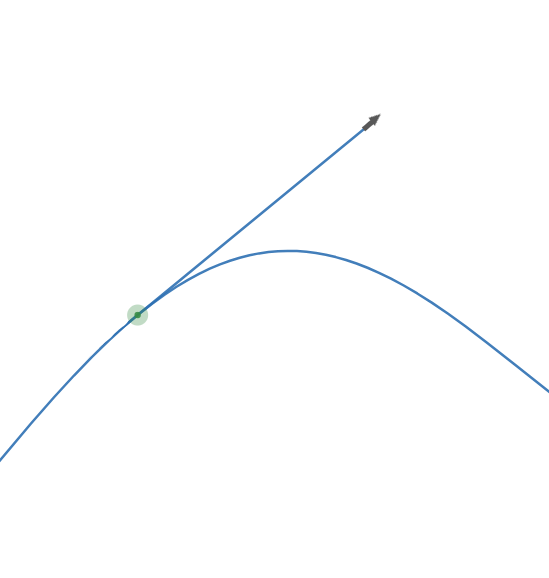
\includegraphics[width=1\textwidth]{image/derivata3}
\caption{Raffigurato il vettore velocità $\vec{v}$}
\label{img:derivata}
\end{minipage}%
\hspace{10mm}%
\begin{minipage}[c]{0.45\textwidth}
\centering
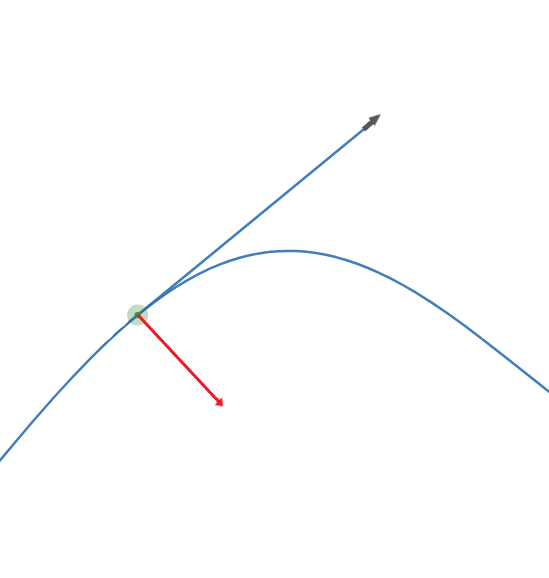
\includegraphics[width=1\textwidth]{image/accelerazione}
\caption{Raffigurato il vettore accelerazione in rosso $\vec{a}$}
\label{img:accelerazione}
\end{minipage}
\end{figure}


\subsection{Cinematica Unidimensionale}

\paragraph{}
La cinematica unidimensionale studia il movimento di un corpo lungo una retta fissando un'origine, chiamata O, un verso di percorrenza e un'unità di misura.

In questa parte trattiamo i due moti rettilinei:
\begin{itemize}
    \item \textit{Moto rettilineo uniforme}
    \item \textit{Moto rettilineo uniformemente accelerato}.
\end{itemize}

\paragraph{}
\subsubsection{Moto rettilineo uniforme:}
Il \textit{moto rettilineo uniforme} è caratterizzato da avere \textit{velocità costante} e \textit{accelerazione uguale a zero}.
\paragraph{}
\textbf{Legge oraria:}
\begin{equation}
    x(t) = x_0 + \vec{v}\Delta t
    \label{leggeOrariamrUnivrome}
\end{equation}

\paragraph{}
Se volessimo rappresentare sul piano cartesiano, in funzione del tempo e dello spazio, questo moto risulterebbe essere una retta nel primo quadrante.

Sull'asse delle ascisse inseriamo la variabile indipendente : $\vec{t}$, mentre sull'asse delle ordinate inseriamo lo spostamento effettuato: $x$. Figura \ref{img:motorettuniforme}.

In Figura \ref{img:TIKZmotorettuniforme} vediamo la relazione tra spazio percorso, velocità costante e accelerazione nulla. Essendo l'accelerazione di questo moto costante, immaginando di essere nello spazio, il corpo continuerebbe con una certa velocità a viaggiare nello spazio percorrendo in ogni $\Delta t$ il medesimo spazio.  
\paragraph{}

\begin{figure}[H]
\centering
\begin{minipage}[c]{0.40\textwidth}
\centering
\begin{tikzpicture}
\begin{axis}[
    axis lines = left,
    xlabel = $t$,
    ylabel = {$s$},
]
\addplot [
    domain=0:4,
    samples=100, 
    color=black,
]{x};
\end{axis}
\end{tikzpicture}
\caption{Grafico Moto Rettilineo Uniforme}
\label{img:motorettuniforme}
\end{minipage}%
\hspace{20mm}%
\begin{minipage}[c]{0.40\textwidth}
\centering
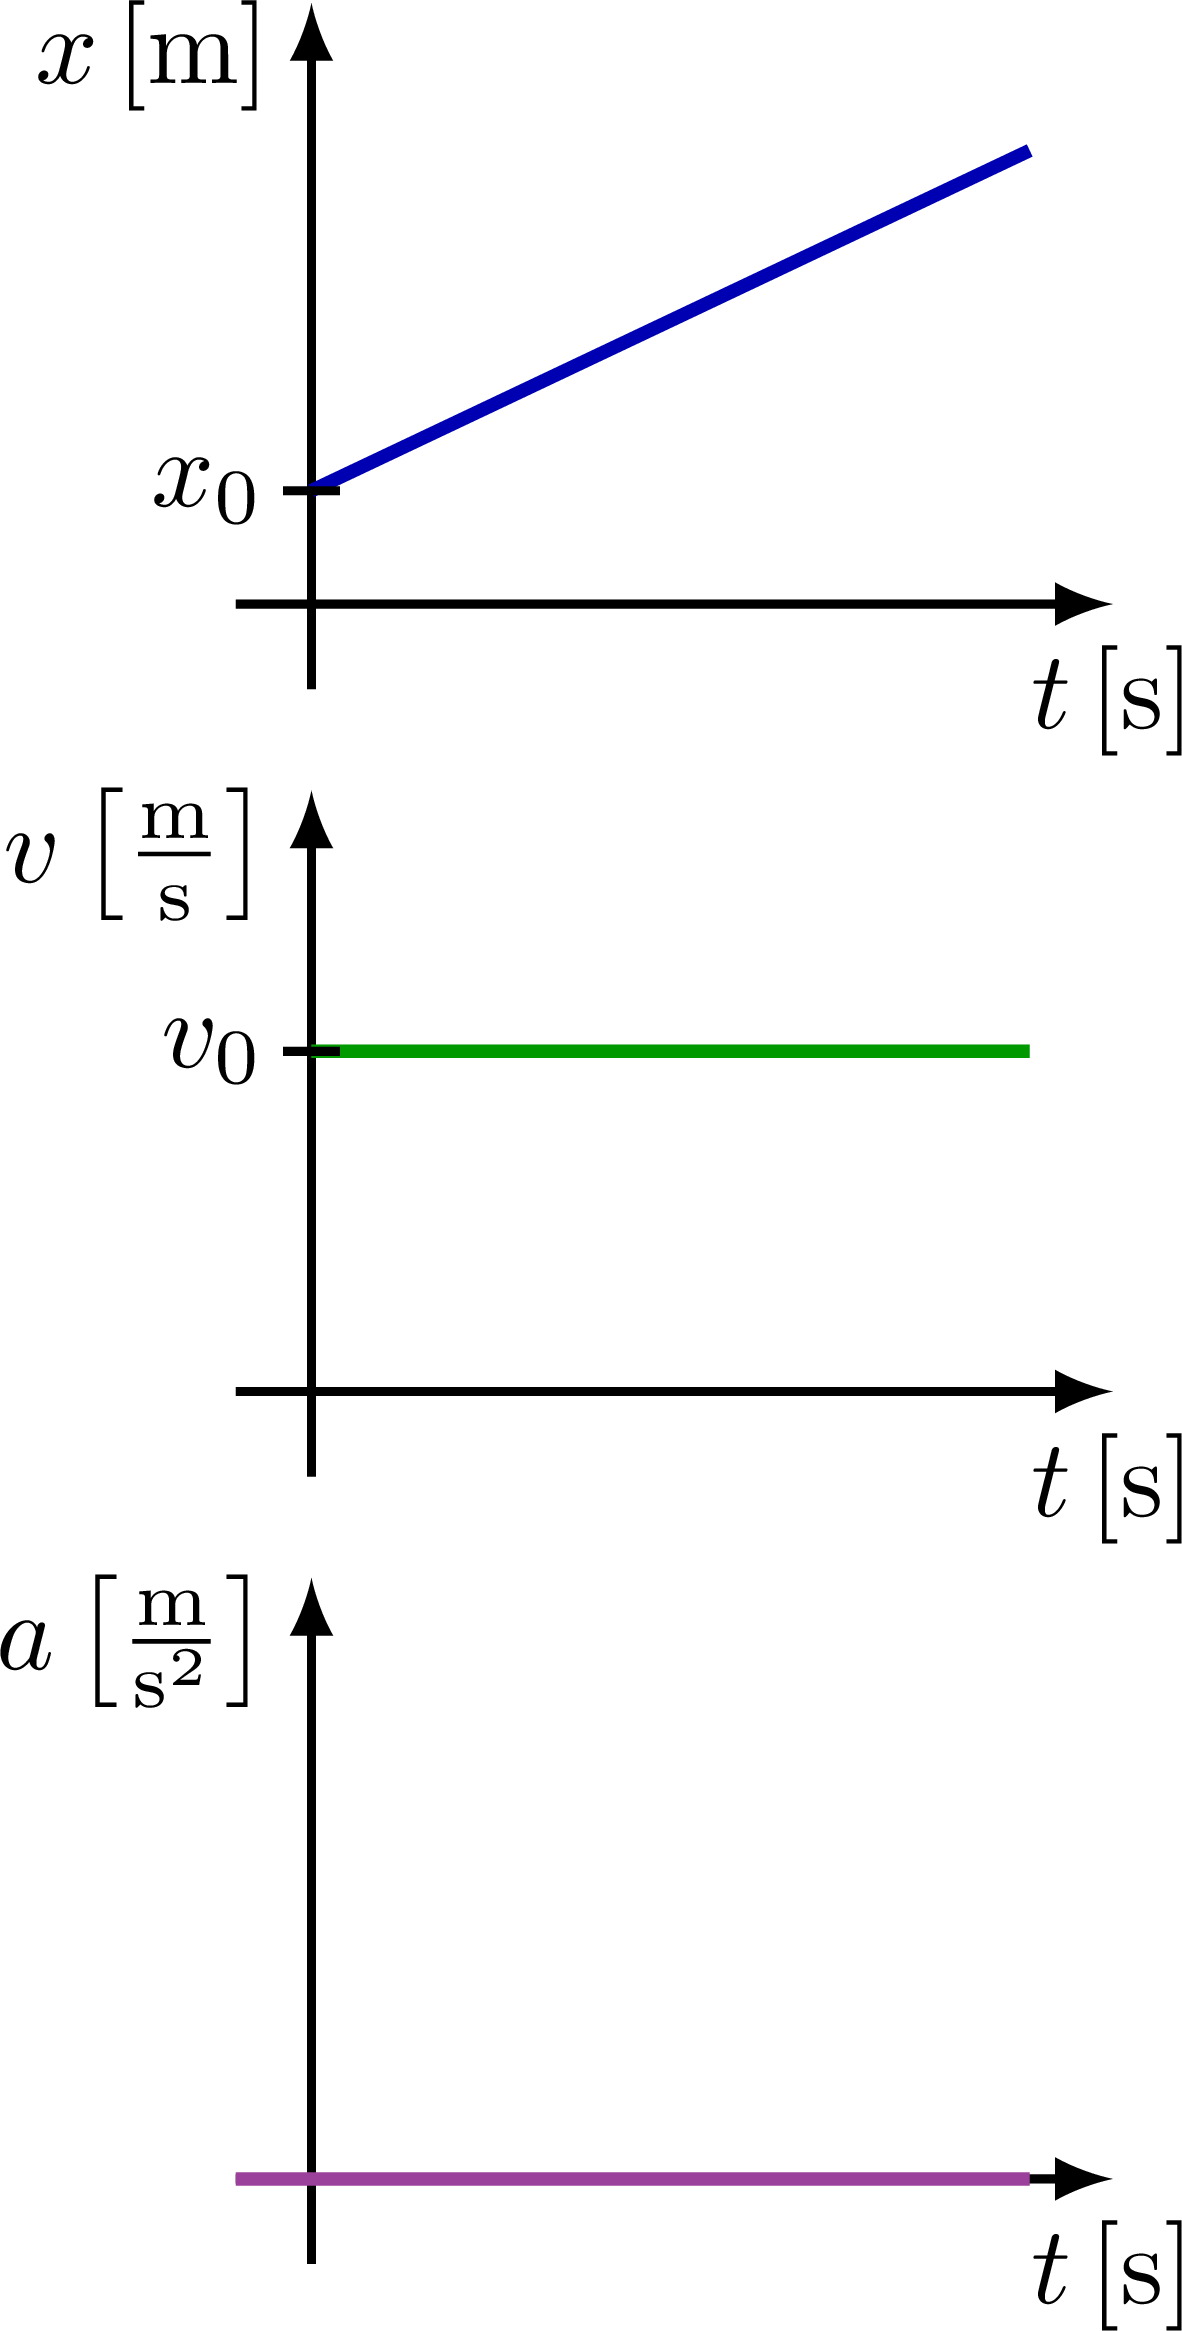
\includegraphics[width=1\textwidth]{image/motoUniforme.png}
\caption{Relazione tra spostamento, velocità e accelerazione}
\label{img:TIKZmotorettuniforme}
\end{minipage}
\end{figure}

\subsubsection{Moto rettilineo uniformemente accelerato:}Un corpo sottoposto a \textit{Moto rettilineo uniformemente accelerato} subisce sempre un'accelerazione costante: si definisce, rispetto al \textit{moto rettilineo uniforme}, un moto vario.

Avendo accelerazione costante $\vec{a}_{cost.}$ la velocità cresce o diminuisce sempre della stessa quantità, quindi in un lasso di tempo vedremo che la variazione di spazio crescerà in maniera quadratica rispetto al tempo.

\paragraph{}
\textbf{Legge oraria:}
\begin{equation}
\label{leggeOrunifacc}
    x(t) = x_0 + \vec{v}_0\Delta t+\frac{1}{2}\vec{a}\Delta t\,^2
\end{equation}
da cui derivano anche:
\begin{equation*}
    \vec{v}=\vec{v_0} + \vec{a}\Delta t \qquad{} \vec{v}\,^2 = \vec{v_0}^2 + 2\vec{a}\Delta x
\end{equation*}
\paragraph{}

Essendo questo moto accelerato costantemente, osserveremo che sul grafico ad ogni unità di tempo lo spostamento sarà sempre maggiore dettato dal fatto che la velocità continua a crescere uniformemente via via che scorre il tempo. Figura \ref{img:motorettuniformementeacc}.
La figura \ref{img:TIKZmotoUniformementeAcc} mostra un corpo che inizialmente ha velocità negativa ma ad un certo istante $t$ cambia direzione, mantenendo sempre velocità constante.


Si pensi ad un pallone lanciato verso l'alto. Inizialmente avrà una velocità data dallo sforzo compiuto dalle nostre braccia per lanciarlo in alto. Sul pallone però agisce fin da subito l'accelerazione gravitazionale la quale farà si che perderà velocità, fino a raggiungere l'altezza massima dove si fermerà, ed inizierà la sua caduta verso il centro della terra. 


\begin{figure}[H]
\centering
\begin{minipage}[c]{0.40\textwidth}
\centering
\begin{tikzpicture}
\begin{axis}[
    axis lines = left,
    xlabel = $t$,
    ylabel = {$s$},
]
\addplot [
    domain=0:4, 
    samples=100, 
    color=black,
]{0.2*x^2};
%\addlegendentry{\(x\)}
\end{axis}
\end{tikzpicture}
\caption{Moto Uniformemente Accelerato}
\label{img:motorettuniformementeacc} 
\end{minipage}%
\hspace{20mm}%
\begin{minipage}[c]{0.40\textwidth}
\centering
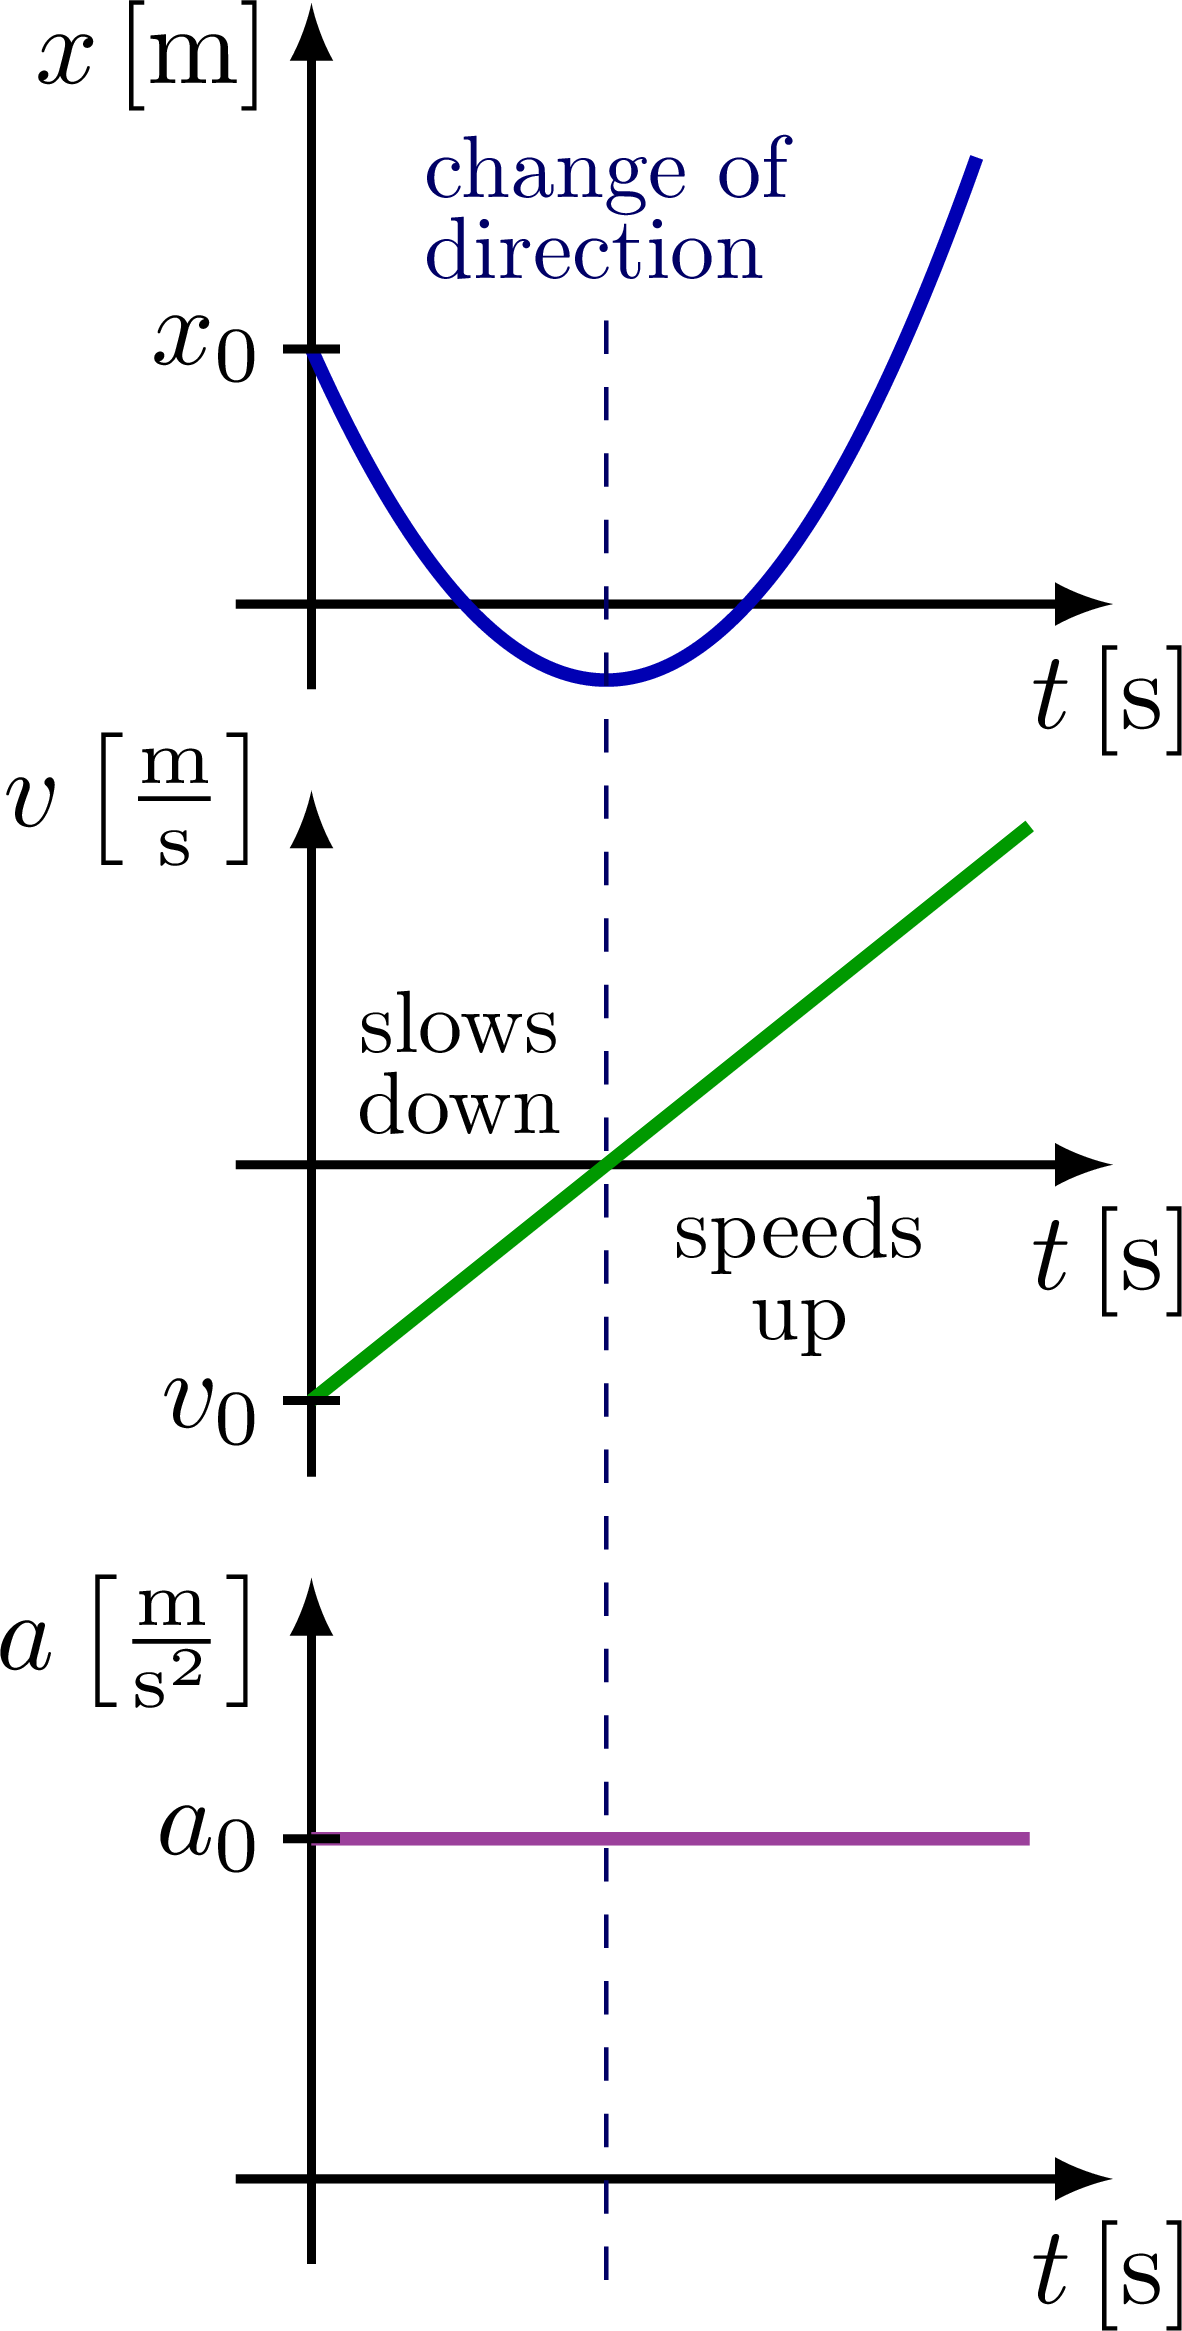
\includegraphics[width=1\textwidth]{image/motoUniformementeAcc.png}
\caption{Inversione di direzione}
\label{img:TIKZmotoUniformementeAcc}
\end{minipage}
\end{figure}

\subsection{Cinematica Multidimensionale}
Per rappresentare le coordinate in un sistema di riferimento cartesiano esistono due metodi:
\begin{itemize}
    \item coordinate cartesiane
    \item coordinate polari
\end{itemize}

\paragraph{}
In \textit{coordinate cartesiane} un punto è rappresentato come combinazione lineare di due vettori: uno posto sulle ascisse e l'altro sulle ordinate. Figura: \ref{coordinateCartesiane}.
\begin{equation*}
    \vec{r} = x\vec{i} + y\vec{j}
\end{equation*}

\paragraph{}
In \textit{coordinate polari} un punto è rappresentato da un versore ortonormale e un angolo $\theta$. Figura: \ref{img:coordPolari}.
\begin{equation*}
    \vec{r} = \vec{r}\,\vec{u}_r \quad,\quad{} dove \qquad{}\vec{u}_r  = \cos({\theta})\vec{i} + \sin({\theta})\vec{j}
\end{equation*}

\begin{figure}[tb]
\centering
\begin{minipage}[c]{0.50\textwidth}
\centering
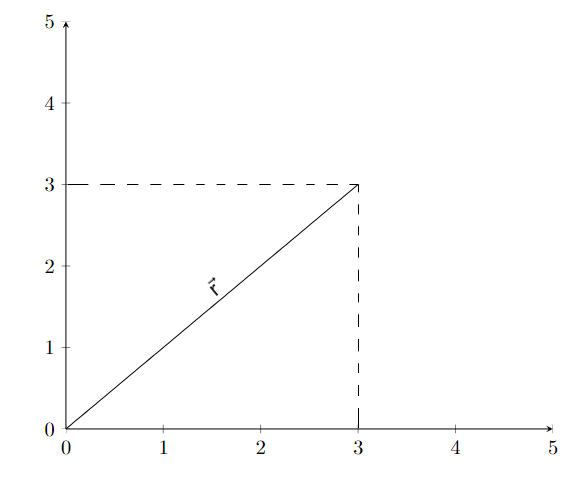
\includegraphics[width=1\textwidth]{image/ccartesiane}
\caption{Piano cartesiano}
\label{coordinateCartesiane}
\end{minipage}%
\hspace{0mm}%
\begin{minipage}[c]{0.50\textwidth}
\centering
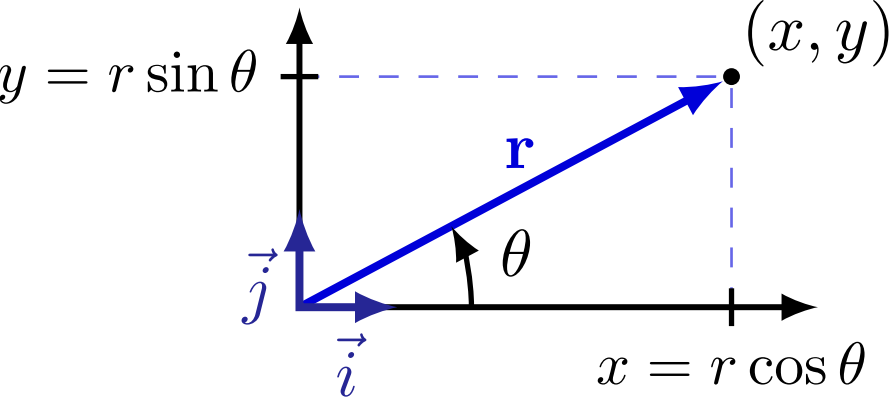
\includegraphics[width=1\textwidth]{image/coordPolari2.png}
\caption{Coordinate polari}
\label{img:coordPolari}
\end{minipage}
\end{figure}

\paragraph{}
\subsubsection{Moto parabolico:}
Il \textit{Moto parabolico} gode di due forze che agiscono sul corpo: una forza orizzontale e una forza verticale diretta verso il basso.

La componente orizzontale si muove di \textit{moto rettilineo uniforme}, la componente verticale invece si muove, verso il basso, con \textit{moto rettilineo uniformemente accelerato}, questo dovuto alla forza di gravità.

\paragraph{}
\textbf{Legge oraria:}

$$
\begin{cases}

     x(t) = x_0 + \vec{v}_x\Delta t\\
     y(t) = y_0 + \vec{v}_{y0}\Delta t-\frac{1}{2}\vec{g}\Delta t\,^2
     
\end{cases}
$$

da cui derivano anche:
\begin{equation*}
    y_{max} = \frac{\vec{v}_{y0}\,^2}{2\vec{g}}\,, \quad t_{volo} = \frac{2\vec{v}_{0y}}{\vec{g}}\,, \quad x_{max} = \frac{2\vec{v}_{0x}\vec{v}_{0y}}{\vec{g}} = \frac{2\vec{v_0}\sin(2\theta)}{g}
\end{equation*}


\begin{figure}[H]
    \centering
    \begin{minipage}[c]{0.45\textwidth}
        \centering
        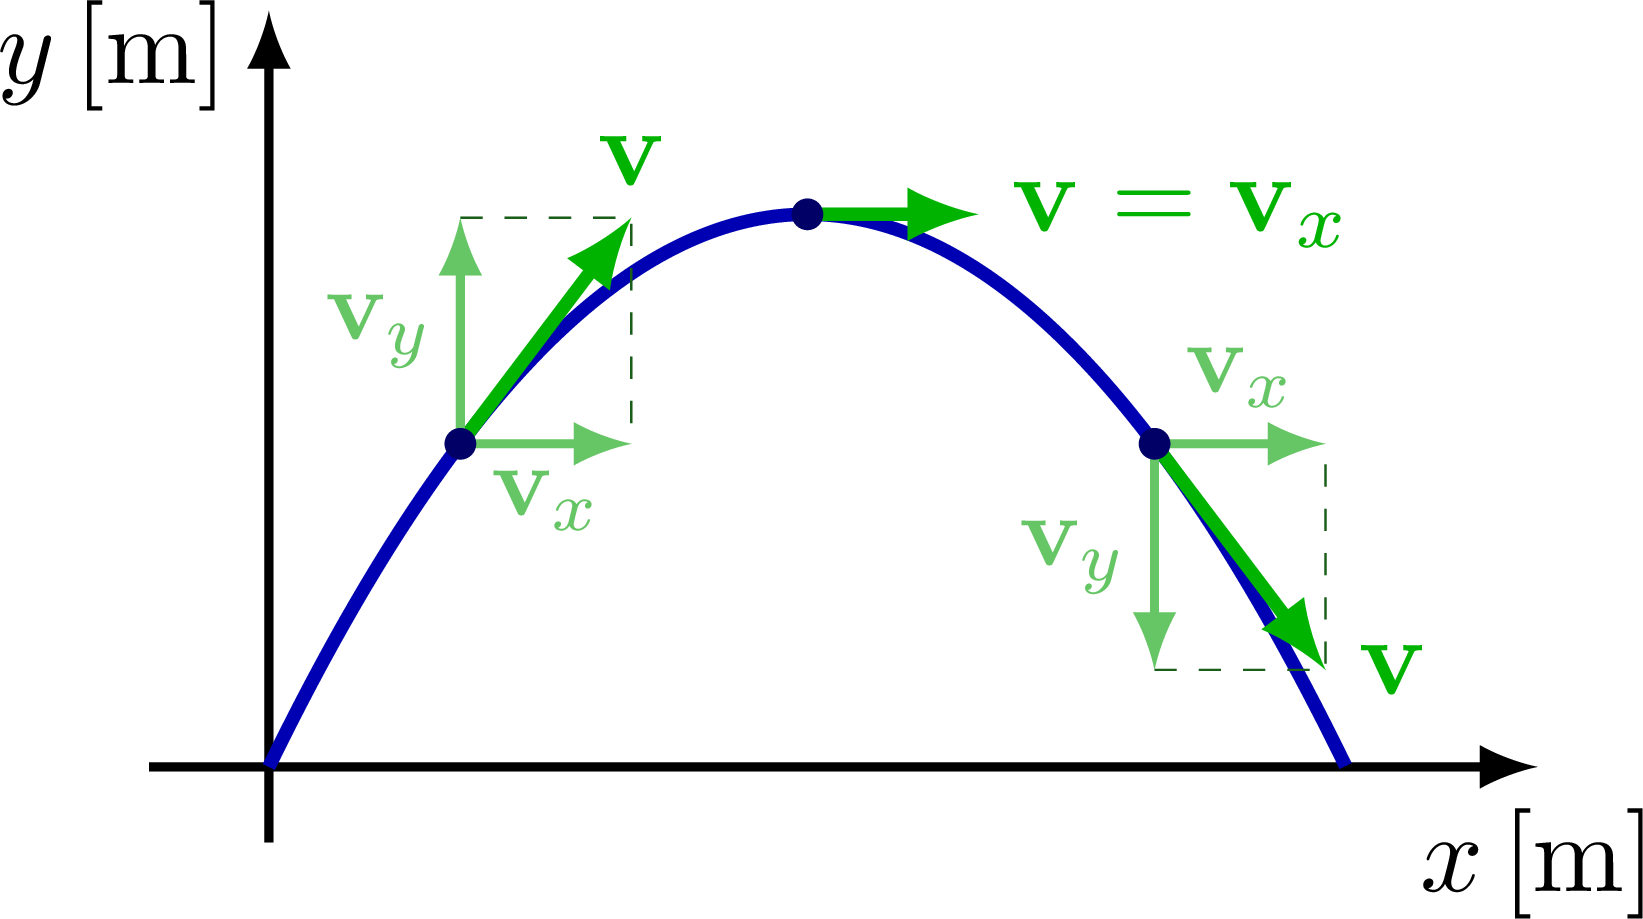
\includegraphics[width=1\textwidth]{image/motoParabolico.png}
        \caption{Moto parabolico}
        \label{fig:motoPara}
    \end{minipage}%
    \hspace{10mm}%
    \begin{minipage}[c]{0.45\textwidth}
        \centering
        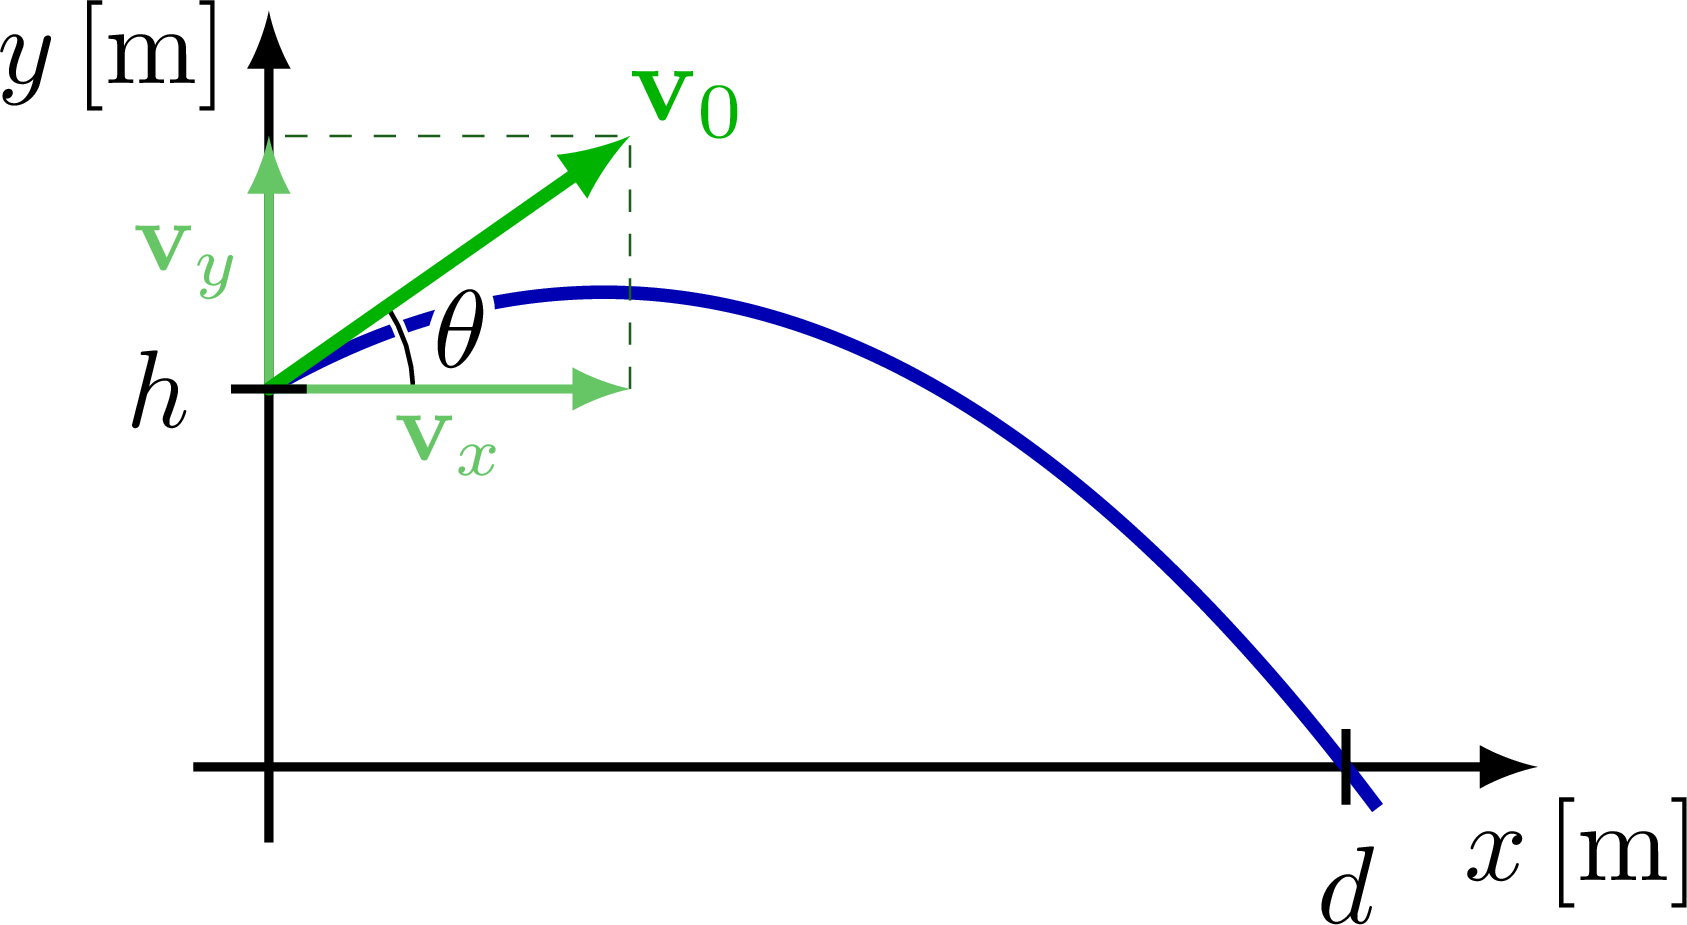
\includegraphics[width=1\textwidth]{image/motoParabolicoinAltezza.png}
        \caption{Moto parabolico da un'altezza h}
        \label{img:motoParaAltezza}
    \end{minipage}
\end{figure}


\subsection{Esercizi}

\subsubsection{Esercizio 1}
Stai guidando un'auto a 66 km/h, e stai avvicinandoti ad un semaforo. A quanti metri al secondo stai viaggiando? [sol: 18,3 $\frac{m}{s}$]

\paragraph{}
Dobbiamo trasformare i  66 km/h in m/s: 
\begin{equation*}
    66km = 66000 m\quad \text{e} \quad h = 3600 s,\quad \text{da cui}\quad \frac{66*1000}{3600} \frac{m}{s} = \frac{66}{3.6} = 18.3\frac{m}{s}
\end{equation*}
\paragraph{}
Ti stai avvicinandoti ad un semaforo. Quando arrivi a 726 m prima del semaforo, il semaforo diventa rosso, ma, un po' per la distanza, un po' per distrazione, impeghi 10.1 s per accorgertene. Appena te ne accorgi, inizi a frenare. A quale distanza ti trovi dal semaforo quando inizi a frenare? [sol: 541.17m]

\paragraph{}
Usando la formula \ref{leggeOrariamrUnivrome} troviamo la distanza percorsa in quei 10,1s di distrazione:

\begin{equation*}
    x = 18.3\frac{m}{s}*10.1s
    x = 184.83m 
    (723-184.83)m = 541.17m
\end{equation*}  

Per trovare la distanza dal semaforo sottraiamo la distanza iniziale con la distanza percorsa in 10.1s:

\begin{equation*}
    (723-184.83)m = 541.17m
\end{equation*}

\paragraph{}
Quale decelerazione devi dare per fermarti esattamente dove si trova il semaforo?[sol: 0.311$\mss$]
\paragraph{}
Usiamo le formule \ref{leggeOrunifacc}
\begin{equation*}
    0^2 = 18.3^2 + 2\vec{a}(541.17)\quad \vec{a} =\frac{(-18.3)^2}{2*541.17}= 0.311\mss
\end{equation*}

\paragraph{}
Quanto impieghi a fermarti, da quando scatta il rosso?[sol: 69,1 s]

Usiamo sempre le formule \ref{leggeOrunifacc}
\begin{equation*}
    18.3\ms=0\ms+0.311\mss*t \quad t =\frac{18.3\ms}{0.311\mss} = 59,1 s \quad (59+10.1)s = 69.1s
\end{equation*}

\paragraph{Esercizio 2}
Romeo si trova sotto il balcone di Giulietta, che è 5.3 m più in alto. Le lancia un messaggio avvolgendolo ad un piccolo sasso, ma un po' troppo forte: così, il sasso arriva più in alto di Giulietta, che non riesce a prenderlo mentre sale... ma riesce a prenderlo quando, scendendo, il sasso cade a 3.1 m/s. A che velocità ha lanciato il messaggio Romeo?

\paragraph{}
Utilizziamo le formule \ref{leggeOrariamrUnivrome} e \ref{leggeOrunifacc}. Uno schizzo del disegno potrebbe essere il seguente: \ref{img:giulietta}

\begin{figure}[tb]
\centering
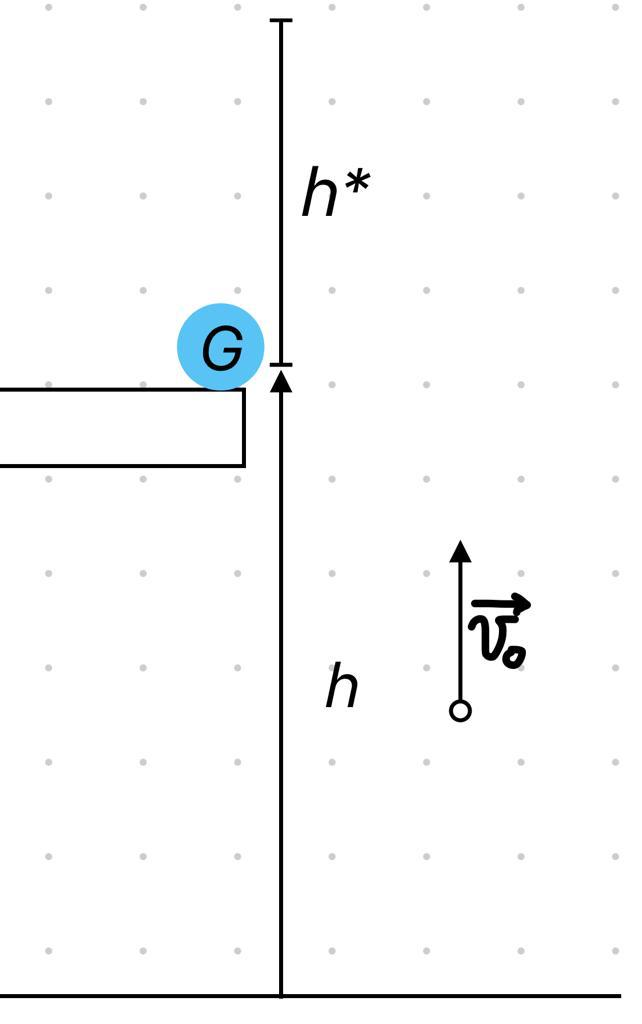
\includegraphics[width=0.30\textwidth]{image/giulietta}
\caption{Esercizio 2}
\label{img:giulietta}
\end{figure}

$$
\begin{cases}
    h + h* = \vec{v}_o - \frac{1}{2}\vec{a}t^2\\
    \vec{v}_ot - at = 0
\end{cases}
$$

Dobbiamo trovare \textit{h*}. Sappiamo che quando arriva all'altezza massima, \textit{h+h*}, la sua velocità sarà pari a zero. Quando poi ricomincia a cadere sappiamo che Giulietta lo prenderà quando il sasso ha una velocità finale di 3.1$\ms$

\begin{equation*}
    \vec{v}_f = \vec{v}_f + \vec{a}t \quad t = \frac{3.1\ms}{9.81\mss} = 0.31s
\end{equation*}

In questo laso di tempo il sasso si sposta di h*, calcoliamolo.

\begin{equation*}
    h* = \frac{1}{2}\veca t^2 = \frac{1}{2}*9.81\mss*(0.31s)^2 = 0.47m
\end{equation*}

A questo punto abbiamo trovato l'altezza massima: 

\begin{equation*}
    h + h* = 5.3+0.47 = 5.77m
\end{equation*}

e possiamo risolvere, mediamte il sistema impostato ad inizio esercizio, la velocità iniziale.

\begin{equation*}
    5.77m = \vv_0t-\frac{1}{2}\vv_0\quad{} => 
\end{equation*}
$$
\begin{cases}
    \vv_o t = 11.54m => t=\frac{11.54m}{\vv_o}\\
    \vv_o = \veca*\frac{11.54m}{\vv_o} => \vv_o\,^2 = 9.81\mss*11.54m => \vv_o = 10.64\ms
\end{cases}
$$

\paragraph{}
A quale velocità avrebbe dovuto lanciare il sasso Romeo perché arrivasse giusto giusto all'altezza di Giulietta?
\begin{equation*}
    0^2 = \vv_o ^2 + 2*9.81\mss*5.3m \quad \vv_o = \sqrt{2*9.81*5.3} = 10.20\ms
\end{equation*}

\paragraph{}
Se avvenisse sulla luna, a quale velocità avrebbe dovuto lanciare il sasso Romeo perché arrivasse giusto giusto all'altezza di Giulietta? E su giove?
\begin{equation*}
    0^2 = \vv_o ^2 + 2*(\frac{9.81}{6})\mss*5.3m \quad \vv_o = \sqrt{2*1.64*5.3} = 4.17\ms\\
\end{equation*}

\text{su giove invece...}

\begin{equation*}
    0^2 = \vv_o ^2 + 2*(\frac{24.79}{6})\mss*5.3m \quad \vv_o = \sqrt{2*24.79*5.3} = 16.21\ms
\end{equation*}


\paragraph{Esercizio 3}
Quale accelerazione deve avere un'automobile, in unità internazionali, per andare da 0 a 54.0 mph in 8.7 s?
mph significa, in inglese, "miles per hour". Un miglio anglosassone corrisponde a 1609 metri. [2.77$\mss$]

Svlogimento.

54mph = 54*1.609 = 86.87km/h = 24.13m/s

\begin{equation*}
    24.13\ms = \veca*8.7s \qquad{} \veca = \frac{24.13\ms}{8.7s} = 2.77\mss
\end{equation*}

Quale frazione di g è questa accelerazione?
\begin{equation*}
    9.81:100 = 2.33:x\qquad{} x = 28\%
\end{equation*}

Quale distanza ha percorso l'automobile , in piedi anglosassoni?[3.28m ]
Un piede anglosassone ("foot") corrisponde a 30,48 cm, e si apprevia con "ft".
\begin{equation*}
    x = \frac{1}{2}*2.77\mss(8.7s)^2 = 104.83m \quad{} 1ft = \frac{1}{0.3048} = 3.28m 
\end{equation*}
\begin{equation*}
    104.84*\frac{1}{0.3048} = 343.96ft
\end{equation*}

Se dovesse frenare decelerando della metà dell'accelerazione iniziale, quanto spazio occorrerebbe per fermarsi?[209.44m]

\begin{equation*}
    \veca = \frac{2.72}{2} = 1.39\mss \quad 0 = 24.13\ms + 1.39\mss t
\end{equation*}
\begin{equation*}
    t = \frac{24.13\ms}{1.39\mss} = 17.36s\quad x = \frac{1}{2}*1.39\mss*(17.36s)^2 = 209.44m
\end{equation*}

\paragraph{Esercizio 4}
Una nuotatrice riesce ad andare a 0,4 m/s quando è in acqua ferma. Sta attraversando  un fiume largo 34 m, con una corrente che scorre a 0,21 m/s. La nuotatrice punta perpendicolarmente all'altra riva.
A quale distanza a valle, rispetto alla perpendicolare, approda all'altra riva?[17.85m] 

Quanto tempo impiega ad attraversare il fiume?[85s]

Con quale angolo dovrebbe dirigersi a monte, rispetto alla perpendicolare alla riva, per attraversare effettivamente il fiume perpendicolarmente alla riva?[32°] 

Quanto ci metterebbe in questo caso ad attraversare il fiume?[96s]
\begin{figure}[tb]
\centering
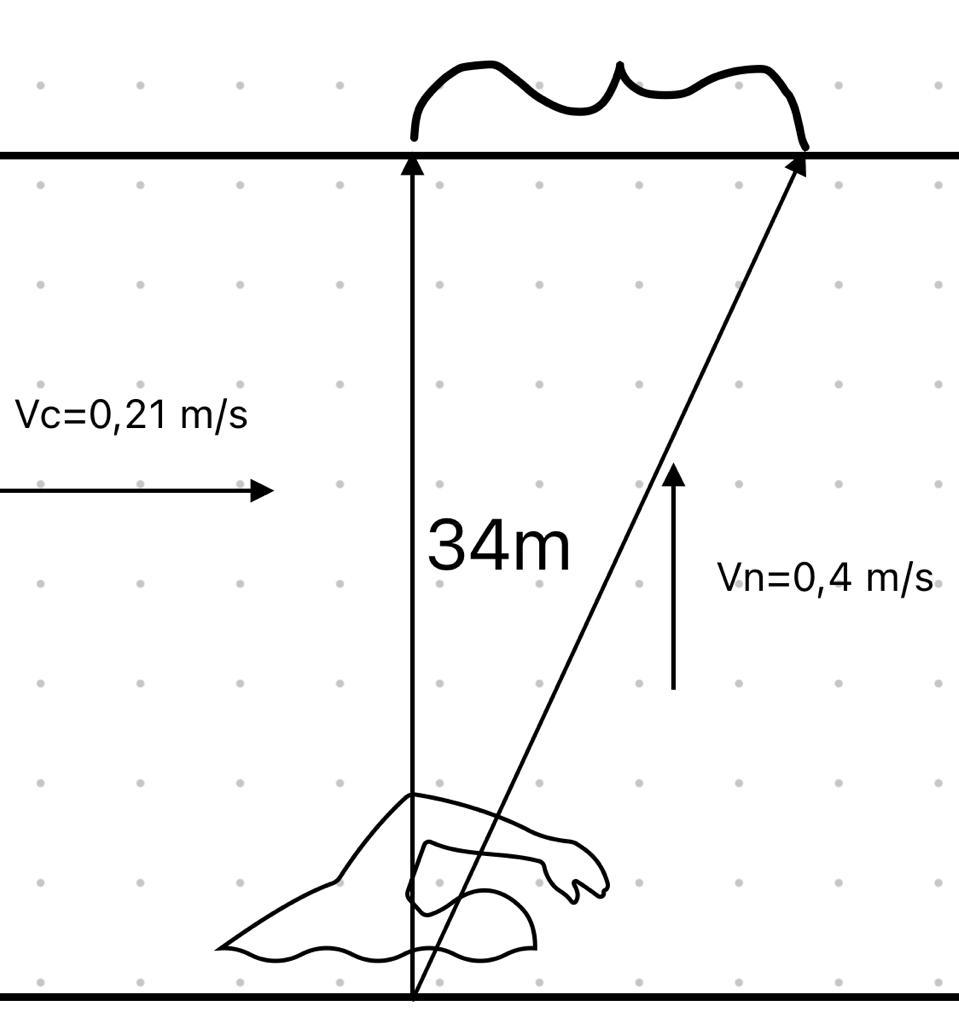
\includegraphics[width=0.45\textwidth]{image/nuotatrice}
\caption{Esercizio 4}
\label{img:nuotatrice}
\end{figure}

\paragraph{Svolgimento:}
 

calcoliamo quanto tempo impiega per attraversare la sponda...
\begin{equation*}
    34m = 0.4\ms t\qquad{} t = \frac{34n}{0.4\ms} = 85s
\end{equation*}
calcoliamo di quanti metri ha spostato la nuotatrice la corrente
\begin{equation*}
    x = 85s*0.21\ms = 17.85m
\end{equation*}

Siccome la nuotatrice mantiene sempre la stessa velocità anche rivolta verso monte allora l'angolo deve essere: 
\begin{equation*}
    0.4\ms \sin{\alpha} = 0.21\ms \qquad{} \arcsin{\alpha} = \frac{0.21}{0.4}\ms = 32\gradi
\end{equation*}

Per rispondere all'ultima domanda troviamo l'ipotenusa del triangolo in figura \ref{img:nuotatrice}:

\begin{equation*}
    ip = \sqrt{17.85^2 + 34^2} = 38.40m\,;\qquad{} 38.40m = 0.4\ms t
\end{equation*}
\begin{equation*}
    t = \frac{38.40m}{0.4\ms} = 96s
\end{equation*}

\paragraph{Esercizio 5}
Un atleta di salto in lungo lascia il suolo con un angolo di lancio di $45\gradi$ rispetto all’orizzontale e atterra a una distanza di 8m. Qual è la velocità di decollo $V_0$ ? 

Adesso sta facendo una corsetta all’aria aperta e giunge sulla riva sinistra di un piccolo fiume. Non c’è un ponte in vista e la riva a destra dista 10 m in orizzontale e 2,5 m in verticale verso il basso. Se l’atleta salta dal ciglio della riva sinistra con un angolo di $45\gradi$ con la velocità calcolata nel punto precedente, quanto dopo o quanto prima atterrerà rispetto alla riva opposta?

\begin{figure}[tb]
\centering
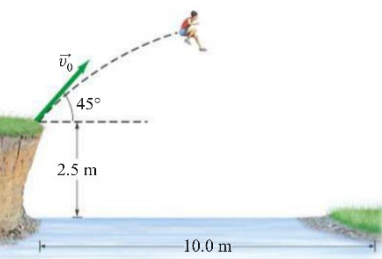
\includegraphics[width=0.45\textwidth]{image/salto}
\caption{Esercizio 5}
\label{img:salto}
\end{figure}




\paragraph{Svolgimento:}

Utilizzando il la legge oraria del moto parabolico avremo che:

$$
\begin{cases}

     x = \vec{v}_0\cos{\theta}t\\
     y = \vec{v}_0\sin{\theta}t-\frac{\vec{g}}{2}t\,^2
     
\end{cases}
$$

ci interessa $V_0$ a noi, troviamo il tempo.

\begin{equation*}
    t=\frac{x}{V_0\cos{\theta}}
\end{equation*}

sostituiamo nella seconda equazione ed otteniamo:


\begin{equation*}
    0 = \frac{xV_0\sin{\theta}}{V_0\cos{\theta}}-\frac{g}{2}\frac{x^2}{(V_0\cos{\theta})^2}
\end{equation*}
\begin{equation*}
    V_0 = \sqrt{\frac{gx}{\sin{2\theta}}} = \sqrt{\frac{9.81*8.0}{\sin{2*45}}} = 8.86\ms
\end{equation*}

Rispondiamo al secondo quesito: 

Osserviamo che ora la distanza del fiume è 10m, sapendo che salta con una  $V_0$ pari a $8.86\ms$ ce la farà o no a raggiungere l'altra sponda?
Siccome nella seconda equazione abbaimo solo il tempo come incognita troviamo il tempo e successivamente sostituiamo nella prima per capire se l'atleta finirà in acqua o si salva da un bel tuffo freddo!


\begin{equation*}
    t = \frac{V_0\sin{\theta}}{g}\Biggl(1+\sqrt{1+\frac{2hg}{V_0^2(\sin{\theta})^2}}\Biggl)
\end{equation*}

sostitendo nella prima\dots


\begin{equation*}
    x = \frac{V_0^2\st\ct}{g}\Biggr(1+\sqrt{1+\frac{2hg}{V_0^2(\st)^2}}\Biggl) = \frac{V_0^2\sin{2\theta}}{2g}\Biggr(1+\sqrt{1+\frac{2hg}{V_0^2(\st)^2}}\Biggl)
\end{equation*}
\begin{equation*}
    x = \frac{8.86^2*1}{2*9.81}\Biggr(1+\sqrt{1+\frac{2*2.5*9.81}{8.86^2*0.5}}\Biggl)= 10m
\end{equation*}

A pelo!

%   MAGARI INSERIRE ALTRI ESERCIZI % 